\section{Materials and Methods}
\label{sec:methodology}

This review follows the PRISMA 2020 reporting guidelines~\cite{Page2021}, the
eight-step SLR process of Xiao and Watson~\cite{XiaoWatson2019}, and the
citation-snowballing protocol of Wohlin et al.~\cite{Wohlin2014}. The completed
PRISMA 2020 27-item checklist is provided as Supplementary Material. The three
intersecting fields covered are parameter-efficient fine-tuning (PEFT) and
adapter architectures; distributed and peer-to-peer (P2P) machine learning;
and multi-task LLM serving and inference. Two AI tools were used in a
strictly advisory capacity (Undermind for candidate retrieval, Claude AI for
abstract-review consistency notes); all inclusion and exclusion decisions were
made by the author. The complete corpus construction pipeline—including
inclusion/exclusion criteria, per-stage counts, tier breakdown, and
bibliometric figures—is documented in
Appendix~\ref{sec:appendix:corpus_pipeline}.

\subsection{Search Strategy and Corpus}
\label{sec:methodology:search}

The search was anchored on nine foundational seed papers (Group G0) selected
for direct cross-pillar relevance and citation impact $\geq$300 in a top-tier
venue. Six thematically focused pre-validated groups (G1--G6) were assembled
by manual curation of leading venues (ACL, EMNLP, NeurIPS, ICML, MLSys);
Table~\ref{tab:groups} summarises their scope and contribution. Forward and
backward citation snowballing on G0 was executed via the Semantic Scholar API
on 2026-04-21, supplemented by a Scopus/WoS forward pass on 2026-05-08.
After deduplication, \textbf{972 unique records} entered title screening,
which merged with the 352-paper pre-validated corpus (G0--G6) to a
\textbf{502}-record corpus. Enrichment and a topical-relevance/tier filter
retained \textbf{464} records. Abstract review across two passes, supplemented
by a forward-citation snowball pass, produced \textbf{552} abstract-reviewed
records; full-text queue selection narrowed these to \textbf{387}, of which
\textbf{190} underwent data extraction, and a manual Scopus/WoS top-up brought
the extraction set to \textbf{224}. Full-text reading and quality assessment
then reduced the corpus to \textbf{123 papers} (2002--2026); these correspond
to \textbf{121 distinct papers}, because two foundational works (LoRA and the
original adapter-based parameter-efficient transfer-learning method) are each
recorded under both their arXiv and Scopus retrieval keys in the reading list.
This funnel is summarised in Figure~\ref{fig:prisma} and traceable record-by-
record through the unified pipeline file (Appendix~\ref{sec:appendix:corpus_pipeline}).

\begin{table}[H]
\centering
\caption{Pre-validated corpus groups: scope, size, and review section coverage.}
\label{tab:groups}
\begin{tabular}{lp{5cm}rrl}
\toprule
\textbf{Group} & \textbf{Theme} & \textbf{\textit{n} pre-val.} &
\textbf{\textit{n} final} & \textbf{Section(s)} \\
\midrule
G0 & Foundational seeds (PEFT, P2P, serving) & 9   & 20  &
\ref{sec:peft}--\ref{sec:adapter_composition}, \ref{sec:inference_systems} \\
G1 & PEFT methods beyond adapters and LoRA   & 59  & 12  & \ref{sec:peft} \\
G2 & Adapter composition for multi-task NLP  & 37  & 15  &
\ref{sec:adapter_composition} \\
G3 & Decentralised and P2P ML systems        & 95  & 11  &
\ref{sec:p2p_federated} \\
G4 & Adapter multiplexing for LLM inference  & 51  & 12  &
\ref{sec:inference_systems} \\
G5 & Routing and MoE for modular PEFT        & 35  & 9   &
\ref{sec:moe_routing} \\
G6 & Federated PEFT for transformer NLP      & 66  & 29  &
\ref{sec:p2p_federated} \\
Other & Manual additions (Scopus/WoS snowball) & --- & 15 & cross-cutting \\
\midrule
\textbf{Total} & & \textbf{352} & \textbf{123} & \\
\bottomrule
\end{tabular}
\end{table}

\begin{figure}[H]
  \centering
  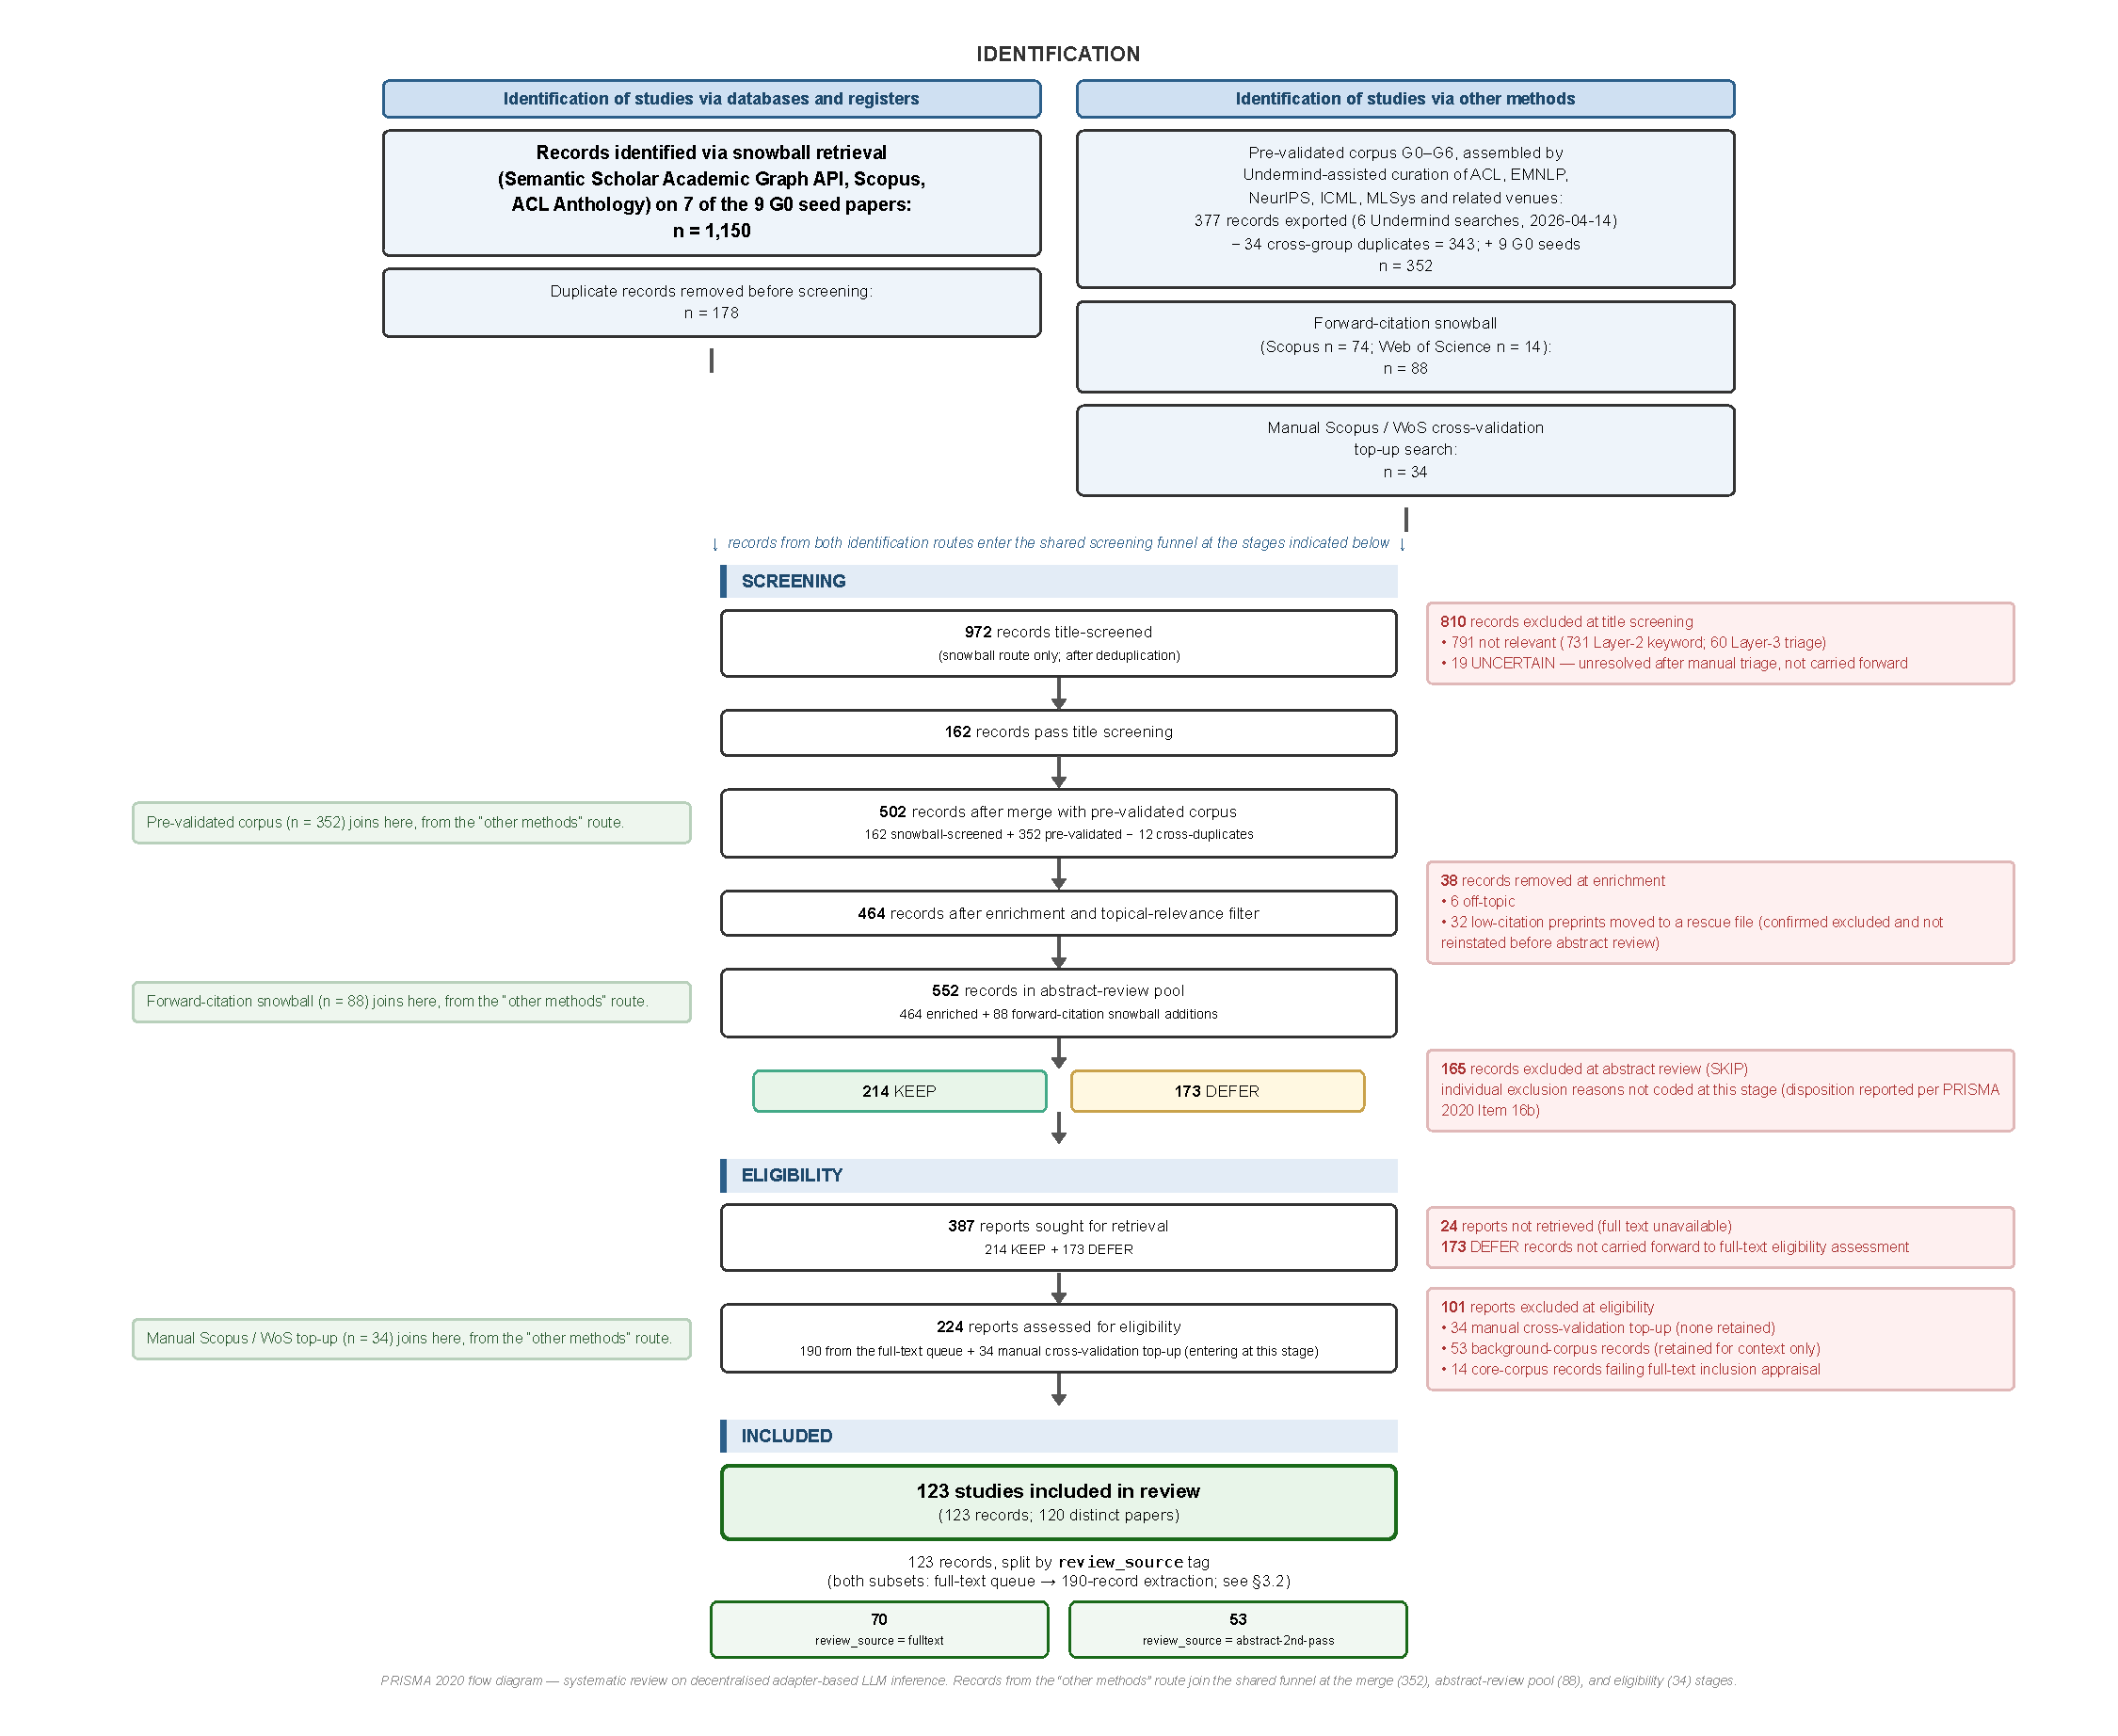
\includegraphics[width=\linewidth]{figures/fig_slr1_prisma_flow.pdf}
  \caption{PRISMA 2020 flow diagram. Records trace from \textbf{1,150} raw
           snowball candidates through deduplication (\textbf{972}), merge with
           the pre-validated corpus and title screening (\textbf{502}),
           enrichment (\textbf{464}), abstract review (\textbf{552}), full-text
           queue selection (\textbf{387}) and data extraction (\textbf{224})
           to the \textbf{123}-paper final reading list (\textbf{121} distinct
           papers).}
  \label{fig:prisma}
\end{figure}

\subsection{Datasets and Benchmarks}
\label{sec:methodology:datasets}

Table~\ref{tab:datasets} reports the datasets, task types, and evaluation
metrics for 33 representative systems drawn from the five synthesis chapters.
PEFT papers predominantly evaluate on GLUE~\cite{WangGLUE2018},
SuperGLUE~\cite{WangSuperGLUE2019}, and MMLU~\cite{HendrycksMMLU2021};
serving papers rely on synthetic throughput benchmarks. No single benchmark
spans all three pillars simultaneously---a fragmentation that is itself one
of the empirical gaps identified in Section~\ref{sec:synthesis_gap}.

\begin{sidewaystable}[p]
\centering
\caption{Selected datasets, tasks, and metrics across the five synthesis pillars.}
\label{tab:datasets}
\small
\setlength{\tabcolsep}{5pt}
  \resizebox{\textwidth}{!}{%
  \begin{tabular}{lllllc}
  \toprule
  \textbf{Paper} & \textbf{Dataset} & \textbf{Task Type} & \textbf{Metric} &
  \textbf{Score} & \textbf{Public} \\
  \midrule
  \multicolumn{6}{l}{\textbf{Pillar 1: PEFT and Adapters}} \\
  Houlsby et al.~\cite{Houlsby2019} & GLUE, SciTail & NLU classification &
  Accuracy & 91.1 (SciTail) & Yes \\
  Hu et al.~\cite{Hu2022} (LoRA) & GLUE & NLU classification & Accuracy & 87.8
  (GLUE avg.) & Yes \\
  Dettmers et al.~\cite{Dettmers2023} (QLoRA) & Vicuna benchmark & instruction
  following & Elo rating & 99.3\% of ChatGPT & Yes \\
  Li and Liang~\cite{LiLiang2021} (Prefix) & E2E, WebNLG, XSUM & NLG & ROUGE-L &
   34.9 (XSUM) & Yes \\
  Ben-Zaken et al.~\cite{BenZaken2022} (BitFit) & GLUE & NLU classification &
  Accuracy & $\approx$ BERT-base full FT & Yes \\
  Poth et al.~\cite{PothAdapters2023} (Adapters lib.) & GLUE & NLU
  classification & Accuracy & matches full FT & Yes \\
  \midrule
  \multicolumn{6}{l}{\textbf{Pillar 2: Adapter Composition}} \\
  AdapterHub~\cite{Pfeiffer2020hub} & GLUE, XNLI & NLU + cross-lingual &
  Accuracy & multiple tasks & Yes \\
  AdapterFusion~\cite{Pfeiffer2021fusion} & GLUE, SciTail, MRPC & NLU
  classification & Accuracy & 96.6 (SciTail) & Yes \\
  MAD-X~\cite{PfeifferMADX2020} & GLUE (6 langs) & cross-lingual transfer &
  Accuracy & zero-shot transfer & Yes \\
  LoraHub~\cite{Huang2023} & BIG-Bench Hard & few-shot transfer & Accuracy &
  34.7 avg per task (BBH) & Yes \\
  LoraRetriever~\cite{ZhaoLoraRetriever2024} & domain QA, MT-bench & multi-task
   QA & Accuracy/win-rate & matches best single & Yes \\
  Ostapenko et al.~\cite{Ostapenko2024} & GLUE, SuperGLUE & NLU classification &
  Accuracy & --- & No \\
  \midrule
  \multicolumn{6}{l}{\textbf{Pillar 3: Adapter-Aware Inference Serving}} \\
  S-LoRA~\cite{Sheng2024} & synthetic & throughput & req/s & up to 4$\times$
  throughput & No \\
  Punica~\cite{Chen2023Punica} & synthetic serving & throughput & req/s &
  12$\times$ higher throughput & No \\
  CaraServe~\cite{Li2024CaraServe} & synthetic & throughput & req/s &
  1.4$\times$ on average & No \\
  Petals~\cite{Borzunov2023} & multiple & instruction following & Accuracy &
  multiple & Yes \\
  MT-EF / {\v{S}}ajina~\cite{Sajina2024} & Reddit, StackOverflow, CoNLL-2003,
  Few-NERD & MTP + NER & Test UA & +11.6\% mean relative gain & Yes \\
  \midrule
  \multicolumn{6}{l}{\textbf{Pillar 4: P2P and Federated Learning}} \\
  FedAvg~\cite{McMahan2017} & CIFAR-10, Shakespeare & image/text classification
   & Accuracy & 10--100$\times$ comm. saving & Yes \\
  FedProx~\cite{Li2020FedProx} & FEMNIST, Sent140 & image/text classification &
   Accuracy & +1--5\% vs FedAvg & Yes \\
  FedPETuning~\cite{ZhangFedPETuning2023} & GLUE & NLU classification &
  Accuracy & $\leq$5\% loss vs central PEFT & Yes \\
  FLoRA~\cite{WangFLoRA2024} & GLUE (few-shot) & NLU classification & Accuracy
  & robust to rank hete. & Yes \\
  DP-FedLoRA~\cite{XuDPFedLoRA2025} & MMLU, BBH, CRASS & NLU + reasoning &
  Accuracy + $(\epsilon,\delta)$ & $\approx$4--5\% loss at $\epsilon=25$ & Yes \\
  SLoRA~\cite{Babakniya2023} & GLUE, SuperGLUE & NLU classification & Accuracy
  & 2$\times$ faster convergence & Yes \\
  Gossip Learning~\cite{HegeduisGossip2019} & synthetic & classification &
  Accuracy & $\approx$ FL quality (20--50\% slower) & Yes \\
  \midrule
  \multicolumn{6}{l}{\textbf{Pillar 5: MoE and Adapter Routing}} \\
  Switch Transformers~\cite{Fedus2022} & C4 pre-training & language modelling &
   Perplexity, speedup & 4$\times$ speedup over T5-XXL & No \\
  Expert Choice~\cite{Zhou2022} & SuperGLUE, WMT & NLU + MT & Accuracy/BLEU &
  +2\% average accuracy & No \\
  DeepSpeed-MoE~\cite{RajbhandariDeepSpeed2022} & GLUE, SuperGLUE & NLU
  classification & Accuracy & 4.5$\times$ speedup, $<$0.5\% loss & No \\
  AdaMix~\cite{WangAdaMix2022} & GLUE, SuperGLUE & NLU classification &
  Accuracy & outperforms single PEFT & Yes \\
  MixLoRA~\cite{LiMixLoRA2024} & GLUE, domain-specific & NLU classification &
  Accuracy & --- & Yes \\
  MiLoRA~\cite{ZhangMiLoRA2024} & commonsense reasoning, math reasoning &
  reasoning + instruction following & Accuracy & $>$ single LoRA & Yes \\
  LoRAMoE~\cite{DouLoRAMoE2024} & world knowledge + instruct & multi-task
  generation & Accuracy, forgetting & alleviates forgetting & No \\
  MOELoRA~\cite{LiuMOELoRA2023} & medical + GLUE & NLU classification &
  Accuracy & $>$ single LoRA & Yes \\
  Crowdsourced MoE~\cite{RyabininCrowdsourced2020} & CIFAR-10/100, MNIST &
  image classification & Accuracy & up to 16 peers, 30\% dropout & No \\
\bottomrule
  \end{tabular}
  }
\end{sidewaystable}
